\chapter{Correcting Masks After the Fact}\label{ch:post}

\section{Introduction}\label{sec:post-intro}
\epigraph{Since all models are wrong the scientist must be alert to what is importantly wrong. It is
inappropriate to be concerned about mice when there are tigers abroad.}{George Box, \emph{Science
and Statistics} \citeyearpar{box1976}}

The masks produced by a model can be edited after the model has run. Such
\keyterm{post-processing} is cheap: it needs no retraining, and it can be tested on cached predictions
in minutes. The one-pixel erosion of Section~\ref{sec:yolo-erosion} was a form of post-processing,
and it was worth three hundredths on the public leaderboard. This chapter follows our many attempts
to find a second improvement of that kind, and explains what their failures taught us.

We begin in Section~\ref{sec:post-rim} by locating the errors in the masks. We then describe learned
methods for redrawing boundaries (Section~\ref{sec:post-refiners}) and methods that need no training
(Section~\ref{sec:post-free}). Section~\ref{sec:post-structure} examines the predictions that fall
just below the matching threshold, and Section~\ref{sec:post-protocol} describes the three-step
protocol that we eventually adopted for testing any repair. Section~\ref{sec:post-summary}
summarises what post-processing could and could not do.

\section{Where the mask error lives}\label{sec:post-rim}
The first question is where the errors are. For 124 matched pairs of prediction and annotation, we
measured the distance of every disagreeing pixel from the annotated boundary
(Figure~\ref{fig:post-rim}). Two thirds of the disagreement lies within two pixels of the boundary,
and three quarters within three pixels. The error is therefore concentrated in a thin
\keyterm{rim} around each object; the interiors of the masks are largely correct. The same
observation motivates Boundary IoU~\citep{cheng2021boundaryiou}, a measure that compares only a thin
band around the boundary of each mask.

\begin{figure}[t]
\centering
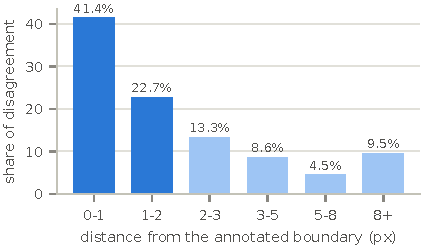
\includegraphics[width=0.62\textwidth]{figures/fig_rim.pdf}
\caption{Where matched masks disagree with their annotations: the share of disagreeing pixels as a
function of their distance from the annotated boundary, over 124 matched pairs.
\generatedby{book/make\_book\_figures.py:fig\_rim}}
\label{fig:post-rim}
\end{figure}

An oracle converted this observation into a score. Removing all of the disagreement within two
pixels of the boundary would raise SQ from about 0.68 to 0.855, and PQ from 0.435 to 0.547 at the
same recognition quality. Removing the disagreement deeper than three pixels instead would raise PQ
only to 0.469. The rim is therefore worth about three times as much as the interior. The deepest band
also showed an unbalanced pattern: beyond eight pixels from the boundary, the model added 5,062
pixels that no annotator drew and missed only 1,384, an over-prediction of 3.7 to 1, whereas every
other band was close to balanced.

How much of the error at the rim can any method remove? The annotators themselves disagree about the
rim. In exp088 we built one mask per filament from the pixel-wise majority of the annotators, and
scored it against \emph{every} annotator of the photograph. It reached a mean IoU of about 0.81, and
the best single annotator's mask reached about 0.80. Our own masks reached 0.68 on the same
photographs. The measured headroom for work on the boundary is therefore roughly the interval from
0.68 to 0.81 in SQ, rather than from 0.68 to 1.

At one point our strategy notes derived an ``SQ ceiling of about 0.82'' by modelling each annotator
as a noisy copy of a hidden true boundary. That model was never tested, and the notes now mark it as
a hypothesis. The measurement of exp088, which scores real masks against real annotators, is the one
to use.

\section{Learned refiners}\label{sec:post-refiners}
The analysis of the rim made a strong case for a \keyterm{refiner}: a second network that takes a
crop of the photograph together with a coarse mask, and redraws the boundary pixel by pixel instead
of trimming every mask by the same amount~\citep{cheng2020cascadepsp,pointrend}. We trained three refiners (Figure~\ref{fig:post-refiner}).

\begin{figure}[t]
\centering
\begin{tikzpicture}[
  st/.style={box=#1, text width=2.35cm, minimum height=1.0cm, font=\sffamily\scriptsize,
             execute at begin node={\hyphenpenalty=10000}}]
  \node[st=inkmuted] (syn) at (0,0.75) {synthetic pairs: annotation dilated, shifted and smoothed};
  \node[st=inkmuted] (real) at (0,-0.75) {real pairs: detector masks matched to annotations};
  \node[st=vizblue, text width=2.6cm, minimum height=1.6cm] (net) at (3.7,0)
       {refiner U-Net on a 256 px native crop; inputs: photograph and coarse mask};
  \node[st=vizorange] (out) at (7.3,0) {refined mask, pasted back at native resolution};
  \draw[flow] (syn.east) -- (net.west |- 0,0.35);
  \draw[flow] (real.east) -- (net.west |- 0,-0.35);
  \draw[flow] (net) -- (out);
  \node[note, anchor=west, text width=2.6cm, align=left] at (8.75,0.75)
       {exp008/009: own task 0.72\,$\to$\,0.85 IoU; PQ $-0.008$};
  \node[note, anchor=west, text width=2.6cm, align=left] at (8.75,-0.75)
       {exp012/018: 0.61\,$\to$\,0.63 IoU; PQ $-0.031$};
\end{tikzpicture}
\caption{The mask refiners. The same crop-level U-Net was trained on synthetic damage and on real
detector errors. The first learned its own task and still lowered PQ; the second learned almost
nothing and lowered it further. \drawnin{book/chapters/ch09\_postprocessing.tex}}
\label{fig:post-refiner}
\end{figure}

\subsection{Training on synthetic damage}\label{sec:post-synthetic}
The first refiner (exp008 and exp009) was trained on pairs made by damaging the annotations: we
dilated, shifted and smoothed them to imitate the errors that we had measured in the detector's
masks. The refiner learned this task well, raising the IoU on its own validation crops from 0.72 to
0.85 after 138 minutes of training on eight TPU cores. Applied to the detector's real output,
however, it lost:
\begin{center}\small
\begin{tabular}{@{}lccccc@{}}
\toprule
configuration & PQ & SQ & TP & FP & FN \\
\midrule
detector, masks untouched & 0.4169 & 0.671 & 829 & 514 & 496 \\
detector and refiner at threshold 0.6 & 0.4322 & 0.673 & 847 & 467 & 478 \\
\textbf{detector and one-pixel erosion} & \textbf{0.4404} & \textbf{0.684} & 845 & 456 & 480 \\
\bottomrule
\end{tabular}
\end{center}
The refiner improved on the untouched masks, but it lost by 0.008 to an operation with no parameters
at all, and on the leaderboard it appeared as 0.35 against 0.36. Our diagnosis was that the
synthetic damage matched the detector's errors in \emph{severity}, that is, in the average IoU of the
damaged masks, but not in \emph{character}. Real errors are correlated with the content of the
image, for example with faint filaments near the limb, or with neighbouring objects that compete for
the same prototypes. A hand-written corruption does not reproduce these correlations.

A small follow-up experiment taught us something about reading numbers. The SQ of the refined masks
(0.673) was lower than that of the eroded masks (0.684), which suggested that the refined masks were
still too wide and that eroding them would help. Eroding the refined masks cost six hundredths. The
refined masks had roughly the right size and the wrong shape. We had read a single scalar difference
as evidence about the \emph{direction} of an error, and it carried no such information.

\subsection{Training on real errors}\label{sec:post-real}
The obvious remedy was to train on real errors. In exp011 we ran the detector over the training
photographs and harvested 3,429 matched pairs of predicted and annotated masks. A refiner trained on
them (exp012 and exp018) raised the validation IoU from 0.611, the IoU of its input masks, to 0.634
at the second epoch, and never improved after that, although its training loss kept falling: it
was memorising the training crops. Scored on the detector's output, it lost 0.031 PQ, because it
rewrote about a third of each mask, and rewrote it wrongly.

\subsection{A second refiner and a resampling artefact}\label{sec:post-v2}
A later refiner (exp091 to exp094), trained on 7,442 harvested proposals, reported an improvement
in IoU of $+0.0118$ on its crops. In exp094 we found that the improvement had been produced by the
measurement itself. Scoring masks at the resolution of the crops, after resampling
them with nearest-neighbour interpolation, raises their IoU by $+0.0117$ even when no model is
involved. When we pasted the refined masks back into the photographs and scored them at the native
resolution, they were slightly \emph{worse} than the originals ($-0.0023$).

The general rule is that we should measure where the metric measures. The competition scores masks
at $2048\times2048$ pixels, after they have been painted into a disjoint set. A score computed at
another resolution, on crops, or on a filtered subset of the instances can change for reasons that
have nothing to do with the method, so every candidate method should be pasted back, painted and
scored with the official metric at the native resolution before its number is believed.

\section{Corrections without training}\label{sec:post-free}
If a network cannot learn to correct the boundary, perhaps a fixed rule can. We tried four
corrections that need no training.

\paragraph{A higher cut on the mask field (exp017).} YOLO turns its continuous field of mask logits
into a binary mask by thresholding it at zero. Raising the threshold moves each boundary inward by an
amount that depends on the local gradient of that mask's own logits. This gives a continuous,
per-instance trim, which the one-pixel erosion is not. As a mechanism it works: with no erosion, a
cut at a logit of 0.9 recovered 0.018 of the 0.023 that erosion recovers. However, it never beat
erosion, and the two do not combine, because they make the same correction. The variation of the
trim from one mask to another did not correlate with how much each mask needed to be trimmed.

\paragraph{Snapping to the intensity edge (exp029).} A filament is dark and the disk is bright, so
the boundary seems to be physically present in the photograph, and one could pull each mask onto it
without any learning, much as an active contour~\citep{kass1988} is pulled onto the edges of an
image. On a synthetic filament drawn as a clean step in intensity, snapping raised the IoU of a mask
that was too wide from 0.80 to 0.9995. On real photographs it destroyed the masks, and the more of
the boundary it was allowed to move, the worse the result. The table also includes a guided
filter~\citep{he2013guided}, which smooths a mask along the edges of the photograph; it changed
almost nothing:
\begin{center}\small
\begin{tabular}{@{}lccc@{}}
\toprule
method & PQ & SQ & RQ \\
\midrule
untouched & 0.4274 & 0.678 & 0.631 \\
guided filter & 0.4276 & 0.678 & 0.631 \\
intensity snap, band of 2 px & 0.3933 & 0.654 & 0.601 \\
intensity snap, band of 3 px & 0.3491 & 0.633 & 0.552 \\
intensity snap, band of 5 px & 0.2739 & 0.621 & 0.441 \\
\bottomrule
\end{tabular}
\end{center}
Figure~\ref{fig:post-profile} shows why. A real filament has no edge. It fades into the disk over
several pixels, and the annotated boundary is a judgement about where the fading stops counting as
filament. The synthetic test had a hard edge built into it, and the existence of such an edge was the
very assumption that the test was supposed to check.

\begin{figure}[t]
\centering
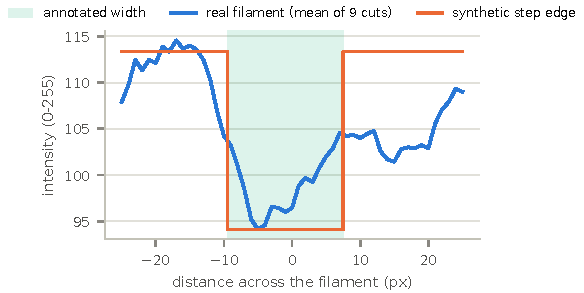
\includegraphics[width=0.66\textwidth]{figures/fig_profile.pdf}
\caption{The intensity across a real annotated filament (the mean of nine cuts perpendicular to its
axis), compared with the step edge that a synthetic test assumed. The real profile fades over several
pixels, so no particular intensity level marks the annotated width.
\generatedby{book/make\_book\_figures.py:fig\_profile}}
\label{fig:post-profile}
\end{figure}

\paragraph{A foundation model (exp066).} We prompted SAM2~\citep{ravi2024sam2}, a general-purpose
segmentation model that extends Segment Anything~\citep{sam}, with the box of each detection, with and without three points inside the mask, and
asked it to redraw the mask. On 24 validation photographs its masks scored 0.358, against 0.459 for
the unchanged masks.

\paragraph{Borrowing another model's boundary (exp072 and exp075).} For each detection that a second
model had also found, we replaced the mask by the second model's mask, or by the intersection or union
of the two. All 640 substitutions lowered the score, which ranged from 0.4529 to 0.4538 against
0.4559 without them.

\subsection{Five failures and an overreach}\label{sec:post-overreach}
By this point five methods had failed to improve the boundary, each approaching it from a different
direction: the refiner trained on synthetic damage, the refiner trained on real errors, the higher
logit cut, the intensity snap, and a crop verifier that we describe in Chapter~\ref{ch:recall}. Our
notes then drew a sweeping conclusion: the annotated boundary is one person's judgement, it cannot be
recovered from the image, and therefore \emph{no} post-processing method can reach it.

The measurements were sound, but the conclusion went beyond them. The failure of five particular
formulations is evidence about those formulations. It does not show that every formulation must
fail, and the notes later marked this reasoning as an unproven generalisation. An independent review
of our later work on repairs made the same point more sharply. Of the sixteen repair approaches on
our list at that time, three had been tested directly, three partially, and ten not at all, and the
review observed that ``demotion by a shared precondition is not refutation''. The next two sections
describe the more careful approach that came out of this correction.

\section{Structural repairs}\label{sec:post-structure}
Chapter~\ref{ch:metric} showed that PQ rewards a prediction that crosses the matching threshold far
more than it rewards an improvement to a mask that already matches. A prediction with an IoU of 0.49
adds nothing to the numerator, whereas at 0.51 it adds 0.51 (Section~\ref{sec:metric-leverage}). The
useful question for post-processing is therefore which masks lie just below the threshold, and what
would push them over it. Improving every mask a little is worth far less.

\subsection{What the near misses look like}\label{sec:post-nearmiss}
In exp105 we built, for each annotation record, the bipartite graph whose nodes are the predicted and
annotated masks and whose edges connect overlapping pairs, and we classified the connected components
of this graph, in the spirit of the error analyses that \citet{hoiem2012} and \citet{bolya2020tide}
made for object detectors:
\begin{center}\small
\begin{tabular}{@{}lcc@{}}
\toprule
component & count & with IoU in $[0.4, 0.5)$ \\
\midrule
one prediction, one filament (1:1) & 953 & \textbf{55} \\
several predictions, one filament (fragments) & 29 & 5 \\
one prediction, several filaments (merge) & 24 & 5 \\
several predictions and several filaments & 4 & 1 \\
filament with no overlapping prediction & 286 & -- \\
prediction with no overlapping filament & 211 & -- \\
\bottomrule
\end{tabular}
\end{center}
Most of the near misses (55 of 66) were simple one-to-one pairs whose masks had the wrong shape,
rather than tangles of splits and merges. These 55 masks were \emph{under}-segmented: the median
near miss lacked 575 annotated pixels and had only 139 extra ones. In exp108 we asked where the
missing pixels were (Figure~\ref{fig:post-nearmiss}). For the near misses, 59\% of the missing
pixels lay beyond the end of the mask along its axis, at a median distance of 10.9 pixels, on bodies
with a half-width of only about 2.2 pixels. For healthy matches, by contrast, 76\% of a much smaller
deficit lay within three pixels of the mask. The near misses were therefore mostly
\keyterm{truncated}, that is, cut short, rather than drawn too thin.

\begin{figure}[t]
\centering
\begin{tikzpicture}[
  truth/.style={line width=7pt, line cap=round, draw=inkmuted!45},
  pred/.style={line width=#1, line cap=round, draw=vizorange},
  pred/.default=4pt]
  % (a) healthy: slightly thin everywhere
  \draw[truth] (0,0) .. controls (0.8,0.5) and (1.6,0.5) .. (2.5,0.1);
  \draw[pred=5pt] (0.05,0.03) .. controls (0.8,0.5) and (1.6,0.5) .. (2.45,0.12);
  % (b) truncated: the mask stops short of the filament's end
  \begin{scope}[xshift=3.6cm]
    \draw[truth] (0,0) .. controls (0.8,0.5) and (1.6,0.5) .. (2.5,0.1);
    \draw[pred=5pt] (0,0) .. controls (0.45,0.3) and (0.9,0.4) .. (1.35,0.38);
    \draw[<->, line width=0.5pt, draw=inkprimary] (1.45,0.6) -- node[note, above=1pt] {10--30 px missing} (2.45,0.35);
  \end{scope}
  % (c) merge: one mask over two filaments
  \begin{scope}[xshift=7.2cm]
    \draw[truth] (0,0) .. controls (0.5,0.3) and (0.9,0.35) .. (1.2,0.3);
    \draw[truth] (1.35,0.28) .. controls (1.7,0.2) and (2.1,0.05) .. (2.5,-0.1);
    \draw[pred=5pt] (0,0) .. controls (0.5,0.3) and (0.9,0.35) .. (1.2,0.3) -- (1.35,0.28) .. controls (1.7,0.2) and (2.1,0.05) .. (2.5,-0.1);
  \end{scope}
  \node[note] at (1.25,-0.55) {(a) healthy match:\\ marginally thin at the rim};
  \node[note] at (4.85,-0.55) {(b) near miss:\\ truncated along the axis};
  \node[note] at (8.45,-0.55) {(c) merge: one mask\\ covers two filaments};
  \draw[truth] (10.35,0.45) -- (10.75,0.45); \node[note, anchor=west] at (10.85,0.45) {annotation};
  \draw[pred] (10.35,0.05) -- (10.75,0.05); \node[note, anchor=west] at (10.85,0.05) {prediction};
\end{tikzpicture}
\caption{Three shapes of error. Healthy matches are slightly too thin near the boundary (a). Most near
misses are truncated: the mask stops well short of the end of the filament (b). A smaller group
merges two annotated filaments into one mask (c). \drawnin{book/chapters/ch09\_postprocessing.tex}}
\label{fig:post-nearmiss}
\end{figure}

\subsection{Triggers: can we tell which masks to repair?}\label{sec:post-triggers}
A repair needs a \keyterm{trigger}, an observable signal that indicates which masks need it, because
at test time we do not know which masks lie just below the threshold. Every trigger that we tried was
weak:
\begin{center}\small
\begin{tabularx}{\textwidth}{@{}lXc@{}}
\toprule
experiment & signal & AUC \\
\midrule
exp105c & mask geometry: elongation, solidity, variation of width, and their combination & 0.42--0.55 \\
exp105c & narrow neck: minimum width over median width (for merges) & 0.71 \\
exp106 & the semantic model's support in a ring around the mask & 0.40--0.64 \\
exp107 & disagreement between two YOLO architectures & 0.57--0.60 \\
exp109 & evidence in a cone ahead of the mask's endpoint & near chance \\
exp110--112 & darkness and ridge orientation along the best path ahead & 0.52--0.62 \\
exp111 & profile of the width along the axis (for merges) & 0.72--0.81 \\
\bottomrule
\end{tabularx}
\end{center}
The \keyterm{AUC}, the area under the receiver operating characteristic
curve~\citep{hanley1982,fawcett2006}, is the probability
that a randomly chosen mask needing repair receives a higher score from the trigger than a randomly
chosen mask that does not; it is 0.5 for a random trigger and 1.0 for a perfect one. Even the best
signal, the width profile with an AUC of 0.81, ran into a \keyterm{precision wall}. There were 24
merged masks among 882, a base rate below 3\%. At any threshold that caught a useful share of the 24,
the healthy masks caught alongside them outnumbered them several times over. Experiment exp108 also
explained why the triggers based on a ring around the mask had failed: they sampled a band four pixels
wide around the mask, whereas the missing pixels of a truncated mask lay 10 to 30 pixels beyond its
end.

\section{A protocol for repair experiments}\label{sec:post-protocol}
We had rejected several of these repair ideas because their triggers failed. That was an error of
sequencing: a failed trigger tells us nothing about whether the repair itself is worth anything. The
testing manual that we adopted fixed the order of the questions (Figure~\ref{fig:post-protocol}),
and we introduced it in general terms in Section~\ref{sec:val-oracles}. Here we apply it.

\begin{figure}[t]
\centering
\begin{tikzpicture}[
  st/.style={box=#1, text width=3.0cm, minimum height=1.6cm, font=\sffamily\scriptsize,
             execute at begin node={\hyphenpenalty=10000}}]
  \node[st=vizblue] (a) at (0,0) {\textbf{\color{inkprimary}1. ceiling}\\ an oracle repair that reads the annotations: the family's maximum gain};
  \node[st=vizaqua] (b) at (4.7,0) {\textbf{\color{inkprimary}2. operator}\\ the real repair, told by an oracle exactly which masks to act on};
  \node[st=vizorange] (c) at (9.4,0) {\textbf{\color{inkprimary}3. gate}\\ the real trigger that chooses the masks; its break-even rate};
  \draw[flow] (a) -- node[note, above=1pt] {worth it?} (b);
  \draw[flow] (b) -- node[note, above=1pt] {recovers it?} (c);
  \node[note, text width=3.1cm, align=center] at (0,-1.3) {split: +0.0223\\ lateral growth: +0.0189};
  \node[note, text width=3.1cm, align=center] at (4.7,-1.3) {neck cut: +0.0028 (13\%)\\ dilation: +0.0064 (34\%)};
  \node[note, text width=3.1cm, align=center] at (9.4,-1.3) {dilation needs a gate with\\ TPR / FPR $>$ 3.9};
\end{tikzpicture}
\caption{The protocol for testing a family of repairs. Each step answers one question, and it is run
only if the previous step says that the family is worth pursuing. The numbers come from exp113, exp114
and exp117. \drawnin{book/chapters/ch09\_postprocessing.tex}}
\label{fig:post-protocol}
\end{figure}

\subsection{Step 1: ceilings}\label{sec:post-ceilings}
In exp113 we measured, for each family of repairs, how much a perfect repair could gain if the
annotations were allowed to guide it. Splitting merged masks along the true boundary was worth
$+0.0223$. Growing truncated masks to their true extent was worth $+0.0325$ in total, divided into
lateral growth ($+0.0189$) and axial growth ($+0.0181$), which overlap. Joining fragments was worth
$+0.0116$. Every family passed this first step, and three of them could in principle have lifted our
baseline of 0.4559 above 0.472, the validation score that at the time corresponded to a public score
of 0.40. An oracle ceiling of this kind is an upper bound for research purposes; it can never be
submitted.

\subsection{Step 2: operators under a perfect gate}\label{sec:post-operators}
Given the exact list of masks to repair, how much of the ceiling does a real repair operator recover
(Figure~\ref{fig:post-ceilings})? For splitting, the best rule, a cut across the narrowest point of
the mask's interior, recovered 13\% of the ceiling ($+0.0028$). It rescued 22 of the 40 filaments
that a perfect split rescues, and it damaged 6 healthy matches. A watershed
split~\citep{vincent1991} lost outright. For
growth, the result was surprising: plain dilation, which reads no evidence from the image at all,
beat every growth rule that was guided by the image. Two steps of dilation recovered 34\% of the
lateral ceiling ($+0.0064$), about twice as much as the best grower guided by darkness. Axial growth
along rays from the endpoint of the mask recovered at most 7\% of its ceiling.

\begin{figure}[t]
\centering
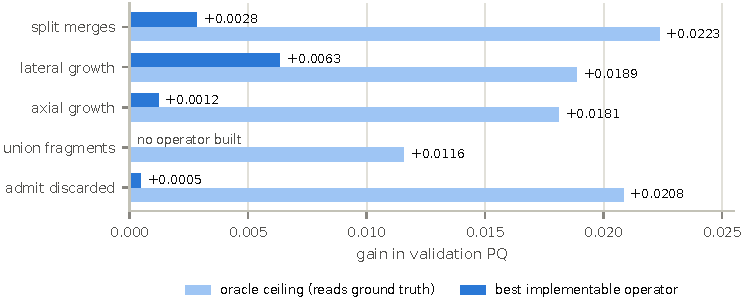
\includegraphics[width=\textwidth]{figures/fig_ceilings.pdf}
\caption{The oracle ceiling of each family of repairs (light), against the best operator that can be
implemented, given a perfect gate (dark). The last row is the admission of discarded candidates
described in Chapter~\ref{ch:recall}. \generatedby{book/make\_book\_figures.py:fig\_ceilings}}
\label{fig:post-ceilings}
\end{figure}

\subsection{Step 3: what a gate must achieve}\label{sec:post-gate}
Comparing an operator with and without its perfect gate reveals what a real gate would have to do.
One step of dilation, applied only to the 55 near-miss masks, pushed 11 of them over the threshold
and harmed none. Applied to all 953 one-to-one masks, it pushed the same 11 over, but it also pushed
43 healthy matches \emph{below} the threshold. Every gain came from the near misses and every loss
from the other masks. Suppose that a gate fires on a fraction TPR of the near misses and on a fraction
FPR of the healthy masks. Since each crossing in either direction changes the score by roughly the
same amount, the expected change is proportional to $11\,\mathrm{TPR} - 43\,\mathrm{FPR}$, and
breaking even requires
\begin{equation}
\frac{\mathrm{TPR}}{\mathrm{FPR}} > \frac{43}{11} \approx 3.9 .
\label{eq:post-gate}
\end{equation}
No trigger in the table of Section~\ref{sec:post-triggers} came close to this ratio at a useful
true-positive rate.

The protocol therefore asks three questions in a fixed order. We first measure the family's
ceiling with an oracle, then measure how much of it a real operator recovers under a perfect gate,
and only then build the real trigger, whose break-even rate we compute from the gated and ungated
runs. A trigger that fails tells us nothing about the value of the repair, and a large ceiling tells
us nothing about whether any practical operator can reach it.

\section{What post-processing could do}\label{sec:post-summary}
Measured carefully, post-processing earned us one large gain and many small losses. The one-pixel
erosion corrected a systematic, uniform bias, and a uniform correction needs no trigger. Every method
that required deciding \emph{which} masks to change stalled, either at the operator or at the gate.
Two facts about the data explain much of this. The error lies mostly at the rim, where the annotators
also disagree, and the near misses are truncations whose missing pixels leave little trace in the
image around the mask. These results do not show that the problem is unsolvable; they show that the
formulations we tested were weak. Our response was to look for a model whose masks needed less repair
in the first place (Chapters~\ref{ch:transformers} and~\ref{ch:training}).

\section*{Exercises}
\begin{exercise}{The rim oracle}
Using Figure~\ref{fig:post-rim}, estimate the gain in SQ from removing all of the disagreement within
one pixel of the boundary, assuming that the disagreement averages 0.472 times the intersection.
Compare your estimate with the gain that the one-pixel erosion actually delivered.
\end{exercise}

\begin{exercise}{Severity is not character}
Write a synthetic damage model whose mean IoU with the annotations is exactly the detector's 0.61.
Propose two statistics of the detector's real errors that your model would fail to reproduce, and
explain how you would measure them on the harvested pairs.
\end{exercise}

\begin{exercise}{Snapping on a real profile}
Take the real profile of Figure~\ref{fig:post-profile}. For each intensity level between its minimum
and its background value, compute the width at which the profile crosses that level. Which level
reproduces the annotated width, and does the same level work for a second filament?
\end{exercise}

\begin{exercise}{The break-even ratio of a gate}
Derive Equation~\eqref{eq:post-gate}, stating the assumption that you make about the value of each
crossing. If each harmful crossing also lowers the SQ of the healthy mask, does the required ratio
rise or fall?
\end{exercise}

\begin{exercise}{The precision wall}
A trigger has an AUC of 0.81 on 24 positives among 882 masks. Assume that the scores of both groups
are Gaussian with equal variance. Find the separation between the two means that gives an AUC of
0.81, and compute the precision at a threshold that catches half of the positives.
\end{exercise}
